\chapter{Instrumentation}
\label{ch:inst}

\par This chapter covers in detail the various pieces of hardware/software which make \vf~possible. 
As with any data processing/search pipeline, the design consists of various components which are intermediated by data buffers. 
Such a design allows for modular component design wherein every component is assigned to be either producer or consumer depending on its position and makes it simplier. This practise is not novel in that it is knownas the \emph{producer-consumer} model.

\par A brief overview of the infrastructure is summarized in~\autoref{ssub:over}. 
The pipeline is graphically described in~\autoref{fig:pipeline}. All the data products/formats are defined in~\autoref{sec:datap}.

\begin{figure}[ht]
	\label{fig:pipeline}
	\centering
	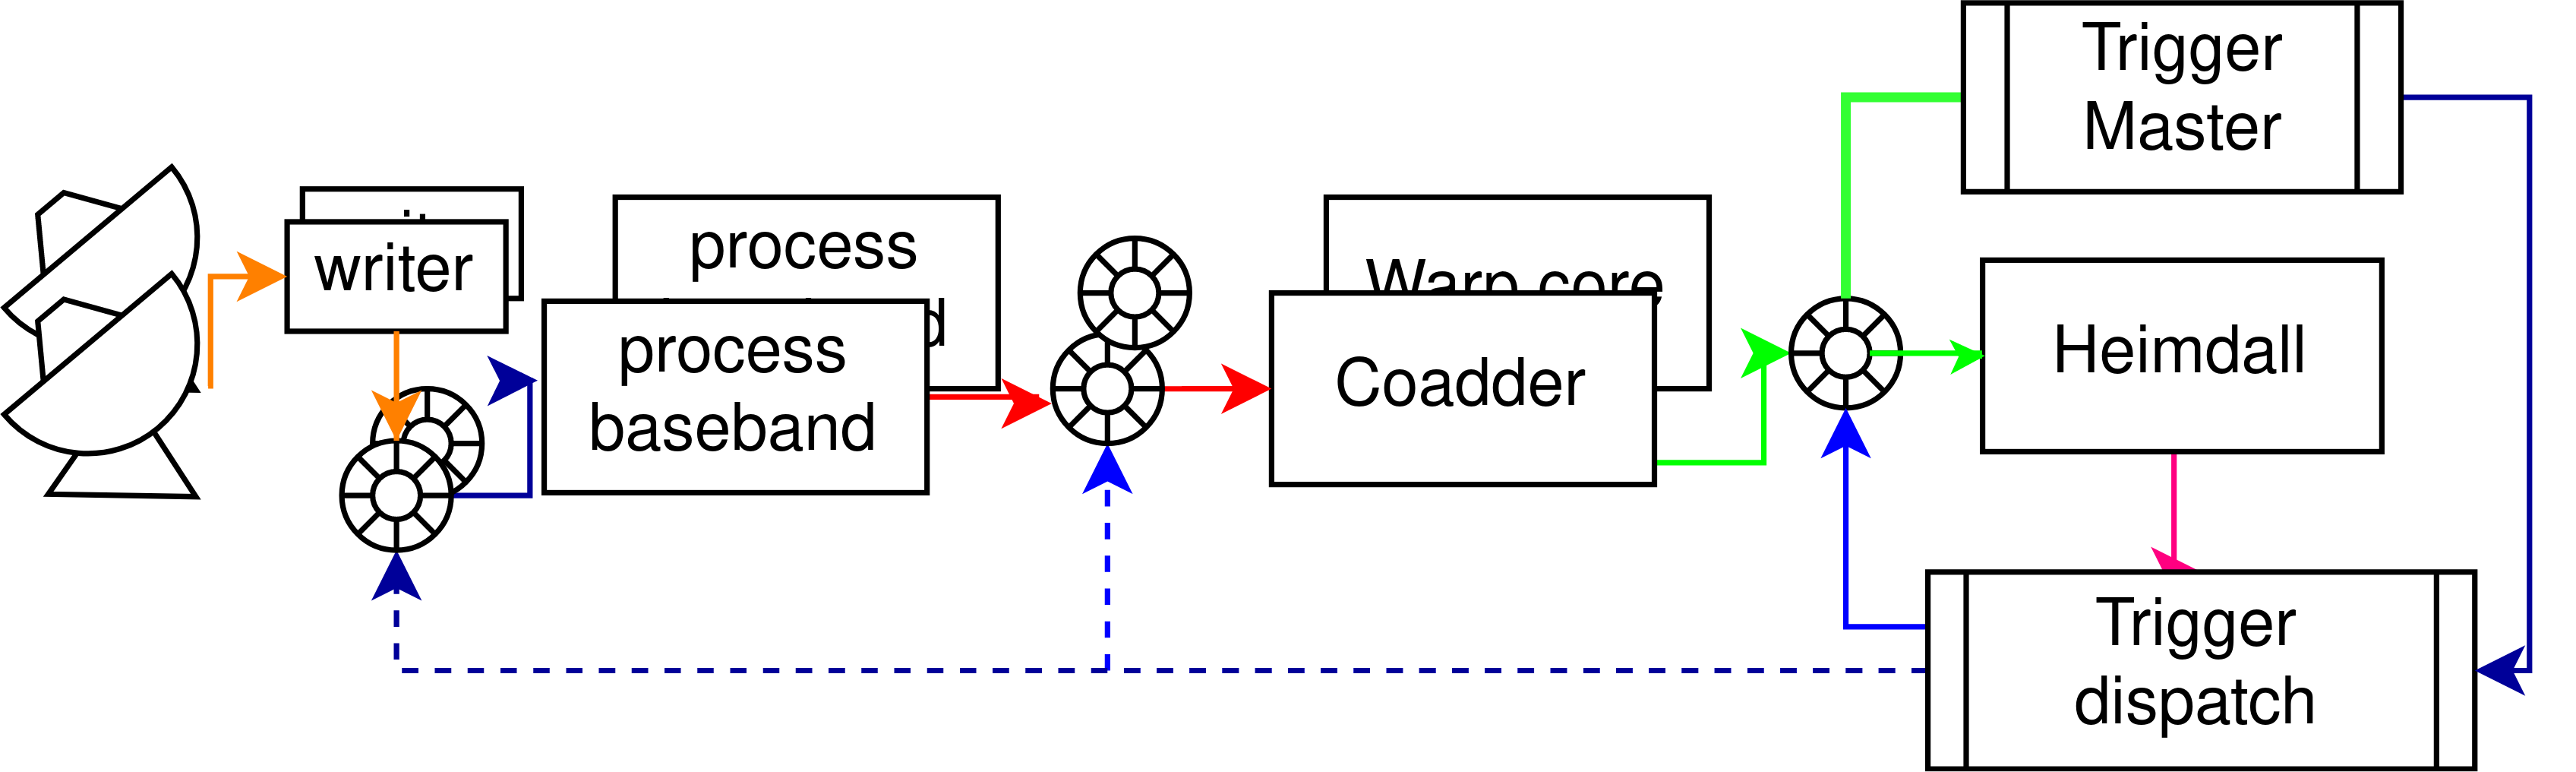
\includegraphics[width=\textwidth, keepaspectratio]{vf_highres.png}
	\caption{\vf~pipeline block diagram. See text.}
\end{figure}

\subsection {Overview}
\label{ssub:over}

\par Firstly, all the components and the data buffers technology are listed and then approached into details in separate sections.
\begin{description}
\item[PSRDADA] Data buffer technology
\item[Writer]  Baseband data packet capturing and writing
\item[Process Baseband] Baseband data to filterbank data
\item[Coadder] Co-adding filterbank data from all antennas
\item[Heimdall] Search program 
\item[Trigger mechanics] Set of python scripts for various trigger level activities
\item[TriggerHook]   Identifies slice of data and copies it for future analysis
\item[TriggerMaster] Realtime trigger responses
\end{description}

\section {PSRDADA}
\par The use of an intermediate buffer is ubiqitious in any real time pipeline. In a producer-consumer model, a producer emits data which is to read by the consumer. 
In a realtime constrained pipeline, the datarates may not be consistent all the time which may lead to consumer waiting for new data (producer is slow), or unable to accept new data (producer is fast).
Hence naturally, many intermdiate buffers are used in \vf~pipeline design.

\par \vf makes use of \dada as an intermediate buffer technology. \dada is built on SYSV shared memory model thus makes use of linux system's kernels and shared memory infrastructure for offering buffering capability. 
\dada codebase is in written in \cc for linux type machines. \dada is versatile that it can support the following modes:
\begin{itemize}
\item Single producer - Single consumer (SPSC)
\item Single producer - Multiple consumer (SPMC)
\item Multiple producer - Single consumer (MPSC)
\item Multiple producer - Multiple consumer (MPMC)
\end{itemize}
Of them all, \vf makes use of SPSC, SPMC oweing for a simple logic which involves a single producer.

\par \dada can be visualized as an $n$-element ring buffer with each ring holding $b$ bytes of data. In addition to the data elements, \dada also offers header blocks which can be used to store data descriptors and such information is stored in ASCII.
Header is defined as key value pair with key being a string and value being any data type.
\autoref{fig:pipeline} shows \dada buffers as the concentric rings made of blocks.

\section {Writer} 
\hfill \emph {The writer code is wholly contributed by Dr. Matthew T. Kerr}

\par \vf is a commensually operated search pipeline. Raw baseband voltage data comes in \texttt{VLBI Data Interchange Format (VDIF)} packets over
\texttt{User Datagram Protocol} network sent by observatory level program called \texttt{executor}. The job of writer is to intercept these data packets and write the header and data into \dada buffer.

\par The raw baseband data consists of two-polarizations, $64$MHz bandwidth real sampled at Nyquist sampling rate of $128$MHz. Writer captures these packets, checks for time ordering and writes into \dada buffer. Time integrity check is of paramount importance since all the following components assume a time continuous flow of data. 

\par Incase writer finds that the incoming packets fail the time continuity check, it is designed to zero fill the packets in between so at least data is continuous in time. The causes for such are many. 
Sometimes, the ethernet network load may be high, or sometimes, the receiving nodes CPU usage is high that it can't respond in time. 
It has also been observed there are some nodes which are more suspectible to packet drops than other nodes. Such nodes are ignored until the underlying issue is resolved. 

\par Another job of writer is to respond to voltage triggers (see~\autoref{sec:tmech}). For every voltage trigger received, writer writes out one second VDIF file, containing packets, to the Solid State Drive (SSD) onboard for the duration of the trigger. Care is taken that overlapping triggers don't cause duplications of raw voltage files.

\section {Process baseband} 
\hfill \emph {The process baseband code contributed by Dr. Matthew T. Kerr}

\par Reading raw baseband produced by \texttt{writer}, \texttt{process\_baseband} hereafter, \texttt{pb}, performs the following operations to output filterbank data into another \dada buffer:

\begin{enumerate}
\item Channelization using Fast Fourier Transform (FFT)
\item Polarization addition
\item Bandwidthing and bandwidth normalization
\item Kurtosis filtering
\item Digitization
\end{enumerate}

\par All the above operations are performed on \texttt{nVIDIA} Graphical Processing Units (GPUs). Channelization uses \texttt{CUDA-FFT (cuFFT)}. 
All other operations involve user kernel launches. Addition of polarization yields Stokes \texttt{I} intesity. The upper edge of the \vf frequency band is polluted by the Mobile Users Operation System (MUOS), hence, the maximum frequency is cut off at $360$MHz bringing the effective bandwidth to $42$MHz. 

\par For a large chunk ($\sim 1$s)of data, the bandpass (time averaged frequency profile) is normalized which removes any frequency variations on the time scales of a second. Since, the signals of interest are much smaller in time and dispersed, such normalization doesn't harm them. In addition to this, there is also a kurtosis based filtering employed which removes any short timescales spurious data.

\par Last operation performed in this component is digitization which digitizes filterbank data with \texttt{NBIT}. Digitization scheme employed follows from~\cite{jenetanderson}. Now, the output data is written to another \dada buffer.

\section {MPI Coadder}

\par Coaddition is the process of averaging time-aligned data streams to produce an averaged data stream. The operation of averaging reduces the noise floor and helps boost the signal.
The motivation for coaddition is firmly established in~\autoref{subs:needcoaddition}. 
\autoref{subs:mpic} explains the workings which make coaddition possible in \vf. 

\par From here on, coadder refers to the component of the \vf which performs coaddition. The underlying technology upon which coaddition operation is based is the Message Passing Interface (\mpi), hence, the coadder is also called \mpi coadder.

\par Coadder reads the filterbank data written to \dada buffer by \pb for all the antennas, coadds, and writes the coadded filterbank data to a \dada buffer residing on a specific node (also called the root node) for further operations. 
In short, the coadder performs, \emph{read-coadd-write} operation in every iteration.

\subsection {Need for coaddition}
\label{ssub:needcoaddition}
\par By the Central Limit Theorem, the distribution of the mean of independent identically distributed (iid) random variables is a Gaussian distribution with mean as the population mean and standard deviation (\sd) as population \sd divided by $\sqrt{N}$.
Noise in the filterbank datastream coming from each of the antenna can be modeled as independent Gaussian noise.
Coaddition reduces the standard deviation of the noise and hence helps in bringing out the signal.
The extent of the attentuation of noise is determined by the sample size i.e, the number of antennas.

\par The signal boosting effect is also established while injecting signals. 
A large amplitude dispersed signal has to be injected in a single antenna to produce the same \sn as in case of coadded antenna.
This will be revisted in~\autoref{ssub:injected}.

\subsection {MPI}
\par Message Passing Interface (\mpi) is a technology ubiqitiously used in all High Performance Computing (HPC) settings. 
\mpi offers various paradigms designed and optimized for parallized jobs. One such paradigm and also the foundational element is the collective algorithm. 
\mpi defines a collective algorithm as one in which all the processes have to participate as a collection, hence the name collective algorithm. Of all the collective algorithms, only two are used in \vf and discussed here:
\begin{description}
	\item[Broadcast] One process has data which it needs to send to every other process.
	\item[Reduce] All processes have data which is to be combined by some operator and the result is to be made available to a process.
\end{description}
In addition to the above collectives (parlance uesd by the HPC community to describe a collective operation), there is also the barrier operation which is used to synchronize processes. 

\par The broadcast operation is performed when one process has data (or message) which is sent to all the other processes. At the end of this operation, all processes have identical data. The reduction operation is performed when all processes have some data which is to combined (or reduced) by some operation. The reduced data is present in a pre-defined process called the \root process. 
The process of coaddition is explained in~\autoref{ssub:coadd}. 

\par \mpi also offers capability of tuning by the Multi Component Architecture (MCA). MCA helps you to configure the various runtime parameters of \mpi jobs from pre-defined options to increase the performance. The tuning options used are described in~\autoref{ssub:tuning}.

\subsection {Coaddition}
\label{ssub:coadd}

\par The operation of coaddition involves summation of the data from all the participating processes followed by a scaling. Naturally, the reduce operation with summation operator is a perfect fit for the summation step. 
The scaling operation can then be performed locally. 
The data is read from \dada buffer (which is written to by \pb). This data has been digitized to \nbit by \pb. 
The first operation of coaddition is to convert the \nbit data into \float data. 
This operation increases the memory footprint by four folds but prevents any overflows in reduce operation and is necessary. 
Next comes the actual \mpi reduce call after which, the coadded filterbank data (in \float) is present in \root process.
The resultant \float is then re-digitized to \nbit and written to a \dada buffer present only on the \root node.

\par Before any reduction is performed, it is paramount to check if all the data are time-aligned. 
This time alignment is checked by the \mjd timestamp of the first datum in the array. 
The \root's timestamp is broadcasted to all the other processes which is then compared against the process's own \mjd timestamp. 
If both the \mjd's match, actual filterbank data is used for reduction otherwise a zero-filled array with the same size as the actual filterbank data is used.

\par The scaling operation done after the \mpi reduce call requires the correct number of antennas which have participated in the collective with real data and not with zero data. 
This is computed by another \mpi reduce operation which is done on a single integer set to $1$ if the process is participating with real data, otherwise set to $0$. This operation reduces the actual number of antennas which have contributed for the coaddition.

\par Coaddition is the major bottleneck of the pipeline and it is also the most computationally expensive step. 
A typical gulp of the data is $8$ seconds which with a typical \nchan{4096}, \nbit{8}, and sampling time amounts to $40$ MB.
Due to the casting to \float, the gulp memory footprint shoots up to $160$ MB.
For a typical number of antennas of $15$, every iteration of coaddition involves $160$ MB of floats summed across $15$ antennas, 
making the total bandwidth of the operation to $160\ {\rm MB} \times 15 = 2.4$ GB.
Naturally, the performance of the pipeline depends on the optimizations of the \mpi operations.
Two of the major optimizations are discussed in the following sub-sections.

\subsection {Reduce}
\label{ssub:reduce}

\par Reduction step is the heart of the coaddition. 
Any sort of delay in the coaddition would hurt the realtime operations of the coaddition. 
Consequently, choice of reduction algorithm was delibrated upon.
The following is heavily relied on the seminal paper~\cite{raben}.

\par The default \mpi algorithm for reduce is the binomial tree reduction. 
The essence of this algorithm is that one process sends it's data and other process receives it and adds it with it's own data.
This repeats until there is only one process. It is graphically visualized to be a binomial tree with individual node's data as the leaves and the reduced data as the root. 
See~\autoref{fig:binreduce}.

\begin{figure}
	\label{fig:binreduce}
	\centering
	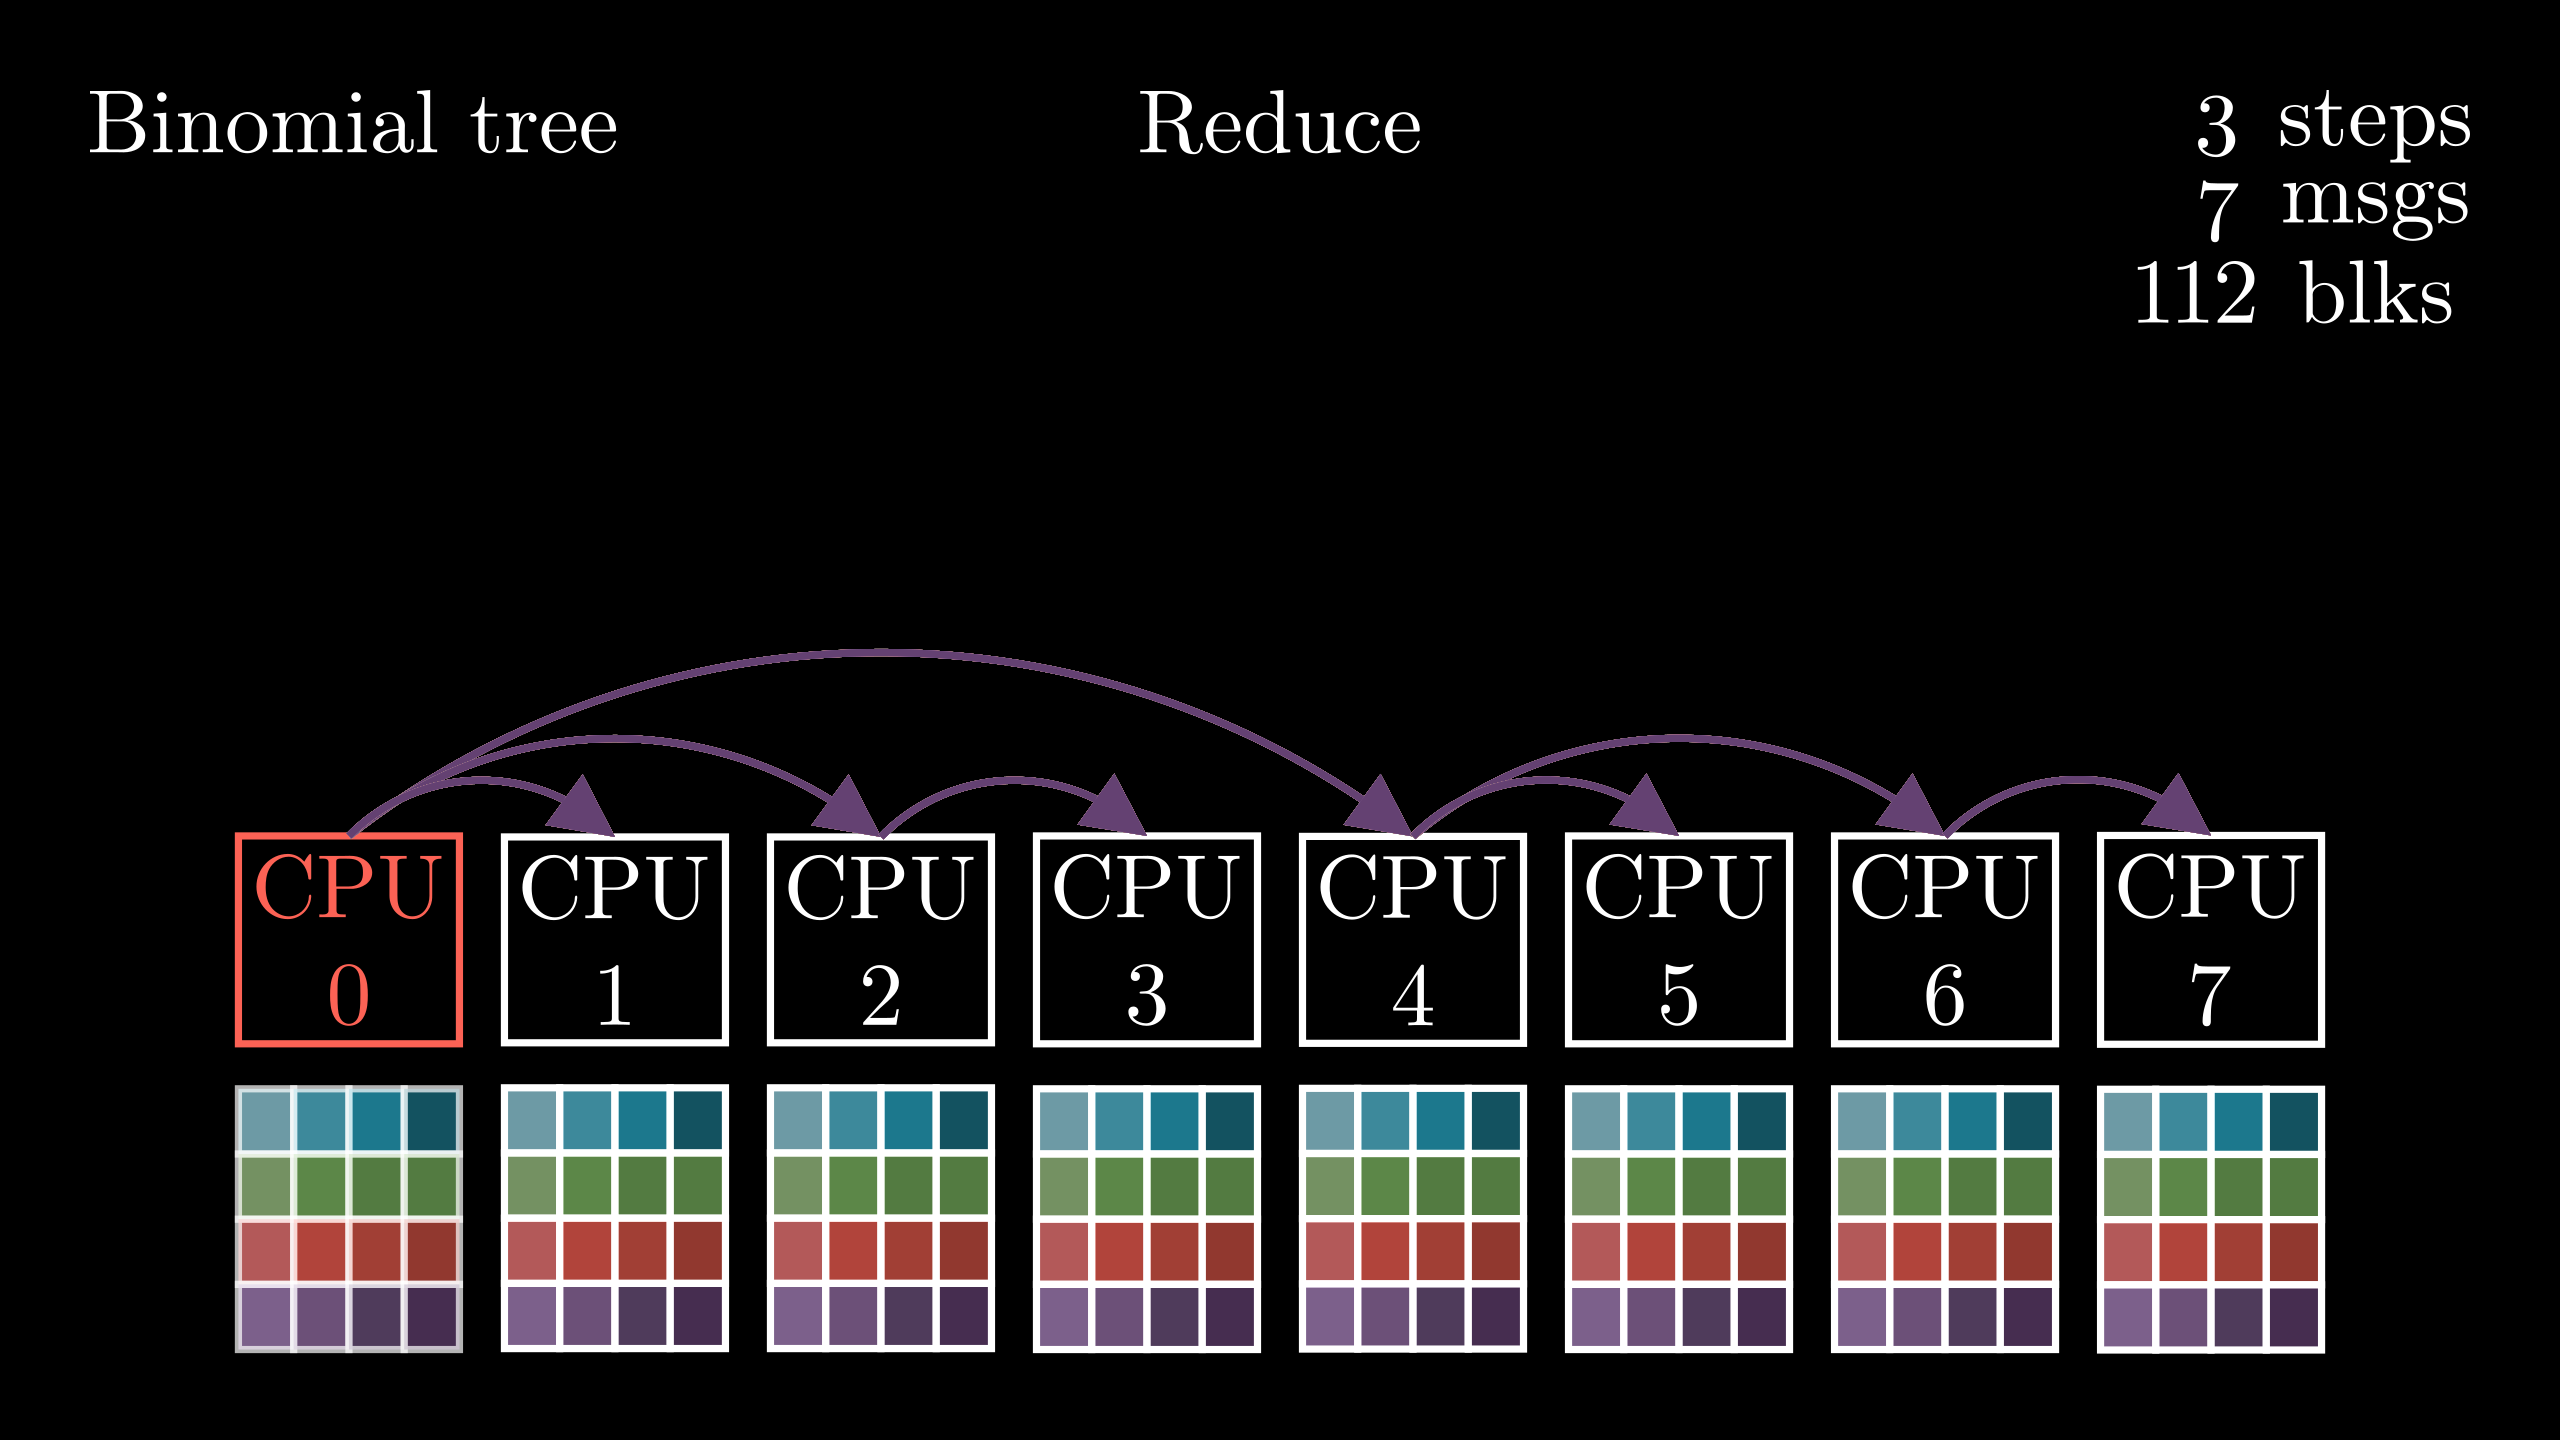
\includegraphics[width=0.8\textwidth,keepaspectratio]{Bcast_Binomial.png}
	\caption{Binomial algorithm for \mpi reduce.(c.f.~\cite{raben}) It looks like an inverted binomial tree, hence, the name.
		This graphic is an frame grabbed from this \href{youtube video}{https://www.youtube.com/watch?v=7gk1a-0sSk8} which is also made by me.
	}
\end{figure}

\par Rabenseifner algorithm~\cite{raben} is an alternate reduce algorithm which is well suited for large messages.
Here, every process instead of reducing the entire message is only responsible for reducing a chunk of the message.
After which, all the processes send their reduced chunk back to root.
The entire process is visualized in~\autoref{fig:rabenreduce}.

\begin{figure}
	\label{fig:rabenreduce}
	\caption{Rabenseifner algorithm for \mpi reduce of large messages~\cite{raben}.}
\end{figure}


\par In order to compare different reduction algorithms, a suitable metric has to be introduced.
Metric employed here is loosely based on~\cite{raben}. 
Two factors govern the metric. One, total number of messages sent. Two, total number of bytes sent.
The former measures the latency which is treated as a constant for any size of message. The latter measures the total bandwidth requirement.
The metrics are only mentioned here. Interested readers are requested to refer~\cite{raben}.
The metrics are tabulated in~\autoref{tab:reducemetric}.

\begin{figure}
	\label{fig:linearshot}
	\centering
	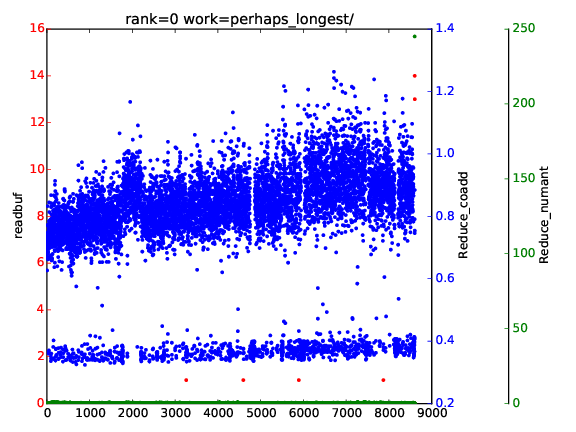
\includegraphics[width=0.8\textwidth, keepaspectratio]{linear_shot.png}
	\caption{The linear trend in \texttt{reduce\_coadd} (shown in blue) as number of iteration increases due to overhead on underlying transport protocol.
		The extremely large \texttt{reduce_numant} (shown in green) is due to the (TCP) transport protocol hanging. See text.
		\texttt{readbuf} (shown in red) is the time taken to a chunk of filterbank data. 
		The x-axis in the plot is the iteration number. For this plot, the \nbit{2} and chunk size was $8$ seconds of data. 
		This is from the early days of \vf~ when $19^h$ was considered a long run, hence the name \texttt{perhaps\_longest}.
	 }
\end{figure}

\par The binomial reduce operation uses less messages but the total number of bytes sent is large. 
It was noticed that 

\begin{table}
\end{table}
% Please add the following required packages to your document preamble:
% \usepackage{booktabs}
\begin{table}[]
	\label{tab:reducemetric}
	\begin{tabular}{@{}llll@{}}
		\toprule
		Name & Latency & Bandwidth & Local \\ \midrule
		Binomial & log N & S & S \\
		Rabenseifner & 2 log N & 2 $\frac{p-1}/p$ S & $\frac{p-1}/p$ S \\ \bottomrule
	\end{tabular}
	\caption{Metric for comparing the different reduce operations. c.f. with~\cite{raben}.
		$N$ is number of processes (or number of antennas) and $S$ is the total size of chunk in each antenna.
		Rabenseifner although has double the latency, the bandwidth is only a fraction, hence is suitable for large messages.
	}
\end{table}

\subsection{Bookkeeping}
\label{ssub:bcast}

% TODO

\par The broadcast of \mjd is a crucial book keeping step. It ensures only time-continuous data goes down the pipeline. 
As discussed above, this is achieved by \root keeping \mjd and other nodes comparing their own timestamp with it.
This operation involves a broadcast

\par In the \texttt{Reduce\_numant} step which computes the number of antennas which have participated in the coaddition,
it was observed that occasionally the the time required would shoot to impossibly large times causing pipeline failure.


\section {Heimdall}

\par The search program employed by \vf is Heimdall(~\cite{heimdall}). 
Heimdall is a Graphical Processing Unit (GPU) based search program which performs multiple de-dispersion trials and tophat matched filtering to identify dispersed signals in the data.
GPUs are needed de-dispersion is extremely computationally intensive operation. 
Heimdall internally uses \texttt{dedisp} (~\cite{dedisp}) for de-dispersion.
Tophat matched filtering helps to boost signals. Lastly, normalization of the time series prior to searching regularizes the data.
A simplified algorithm is shown here:
\begin{verbatim}
	for dm in {2..1000} 
	do
		for iwid in {1..6}
		do
			 de_disperse (dm) 
			 matched_filter (pow (2, iwid))
			 normalize
			 find peaks
		endfor
	endfor
\end{verbatim}

Heimdall in reality is much more sophisticated and performs channel masking, and Radio Frequency Interference (RFI) excision. Interested readers are encouraged to read~\cite{heimdall}.

\par Heimdall reads from the \dada~buffer to which coadder writes the coadded data stream. 
It reads a gulp size of data at a time (a parameter optimized, set to $24$ seconds) and performs multiple
\dm-width trials, if the peaks in the resulting de-dispersed, matched-filtered time series data is significant and over a threshold, 
a candidate is registered at that particular \dm~,width, and epoch.
Heimdall sends out these candidates over to Python server running on the login node from where it is suitably acted upon (discussed in the following sections). 
Additionally, Heimdall also writes out the candidates to a candidate file. See~\autoref{ssub:candfile}.

\section {Trigger mechanics}
\label{sec:tmech}

\par Trigger is a terminology used to denote a candidate which qualifies certain selection rules and warrants follow up action. Trigger mechanics involve receiving triggers from Heimdall, applying selection logic, and performing follow up logic. 
There are two types of triggers: 
\begin{enumerate}
	\item Voltage trigger
	\item DBSON trigger
\end{enumerate}
Voltage trigger, as the name implies, triggers raw baseband voltage data. And, \dbson trigger generates a \dbson file for every trigger. The course of action varies depending on the type of trigger. 
\dbson trigger is treated as the default. If a candidate is to be triggered, then it will \emph{always} have a \dbson trigger.
Each trigger has its own distinct multicast group which makes distinction and follow up action simple and well separated.

\par The underlying \struct which is passed around is the same for both the triggers. \autoref{struct:trigger} shows the struct definition. 
\begin{table}
	\begin{tabular}{llll} \toprule
			Index & Name       & Type          & Comments                                               \\ \midrule
			1     & i0         & double        & UTC start epoch of signal                              \\
			2     & i1         & double        & UTC end   epoch of signal                              \\
			3     & sn         & float         & Signal to Noise ratio of the signal                    \\
			4     & dm         & float         & Dispersion Measure of the signal                       \\
			5     & wd         & float         & Width of the signals in seconds                        \\
			6     & peak\_time & float         & Time since UTC epoch start of signal when signal peaks \\
			7     & meta       & char{[}128{]} & Meta information                                      
			\bottomrule
	\end{tabular}
	\caption {Trigger struct definition. Signal here means the signal of interest. See text for more information.}
	\label{struct:trigger}
\end{table}

\par Voltage trigger handling is solely performed by the writer (see~\autoref{sec:writer}). \dbson trigger response is much more sophisticated and will be dealt in the following sub-sections.

\subsection {Trigger dispatch}

\par Heimdall in addition to writing candidate files, also sends candidate data over to server which is called the trigger dispatch. 
The purpose of trigger dispatch is to receive candidates, apply various candidate selection logics, and multicasts triggers over to the compute nodes. 
Trigger dispatch is written purely in Python.

\par Each selection rule consists of cuts on \sn, \dm, and \wd. In practise, multiple rules are used simultaneously. Moreover, special notch filters to target pulses from pulsars are also applied. 
The type of selection rules used and the triggers received are discussed in great detail in \autoref{ch:data}. Hence, only a simple example of a rule is provided here:
\begin{align*}
	{\rm S/N} &\geq 8 \\
	{\rm DM} &\geq 50 {\rm\ pc/cc} \\
	{\rm Width} &\leq 100 {\rm\ ms}
\end{align*}

\par By default, trigger dispatch only sends out \dbson triggers. More stringent set of rules is applied in case of voltage triggers. 
The reason being SSD space required for voltages is much much more than that required for \dbson~s. 
A typical rule for a \dbson trigger to also be a voltage trigger is a simple cut as, \sn $\geq 25$. Such a simple rule allows for any serendiptious voltage triggering on strong triggers.

\subsubsection {Throttling}
\label{sssub:rfim}
\par Dispatching all the triggers received may sometimes overload the pipeline, cause lags, and may ultimately fail the pipeline.
Hence, a suitable trigger throttling mechanism is put in place.
Trigger rate may skyrocket for a multitude of reasons. It may be so whenever a bright radio pulsar in in the field-of-view (FOV) of \vf.
It may also be when Radio Frequency Interference (RFI) is strong, causing a large number of spurious triggers.
Given the frequency band of operation ($320-384$ MHz) being not just close to walky-talkies used by on-site engineers but also being close to MUOS band, \vf~is more suspectible to RFI.
Presence and effects of RFI is discussed more in detail in~\autoref{sec:RFI}. 
Here, only the instrumentation part of the throttling is described.

\par Heimdall performs searches in batches. All the candidates from a batch are sent at once after the batch has been processed.
Throttling is done at a sub-batch level. A typical batch size is $30720$ samples ($\sim 24$ seconds) and the sub-batch is $8$ seconds.
As discussed in~\autoref{sec:RFI}, if a sub-batch sees more than $200$ triggers, it is vetoed against not dispatched.

\subsection {Trigger hook}

\par Any type of follow-up analysis requires the filterbank data spanning for the duration of the trigger. The job of Trigger hook is to receive the \dbson trigger, slice the appropriate filterbank data, and write it along with trigger information into \dada buffers.

\par Input to trigger hook is the same \dada buffer used by Heimdall for its searching. Output of trigger hook are two separate \dada buffers, one for trigger information (header) and one for trigger data (data). 
\dada offers header block in a buffer but the number of headers is hardcoded to $8$ which would severly reduce the number of triggers that can be held in buffer to $8$.  Hence, two separate buffers are employed.

\par Trigger Hook reads the buffer and keeps track of the UTC epochs of the first sample in each data-block as it reads. 
Then, for a trigger received, with some pointer arithmetic, a slice of filterbank data is written to the data \dada buffer and trigger information is written to header \dada buffer.

\par Trigger hook also holds the option to write out a \fbson. But, this option is not typically used since follow up action is performed anyway.

\subsection {Trigger master}

\par Reading from the buffer to which Trigger Hook has written the sliced filterbank along with trigger information, Trigger master performs the following:
\begin{itemize}
	\item Generating: 
		\begin{itemize}
			\item De-dispersed filterbank binary JSON (\dbson, see~\autoref{ssub:dbson})
			\item Trigger plot (see~\autoref{ssub:tp})
		\end{itemize}
	\item Machine learning (ML) based classification of the trigger and baseband triggering.
\end{itemize}

\par The following only discuss the generation of \dbson~and trigger plot. 
The entirity of classification is discussed in great detail in~\autoref{chap:ml}.
Firstly, the bowtie plane is introduced. And

\par The bowtie plane is computed using the Fast De-dispersion Measure Technique (FDMT,~\cite{fdmt}).
The low frequency introduces large delays which make the FDMT algorithm extremely slow. 
Hence, prior to FDMT, the data is first incoherently de-dispersed to first \dm and then FDMT is applied.

\begin{figure}
	\label{fig:bt}
	\centering
	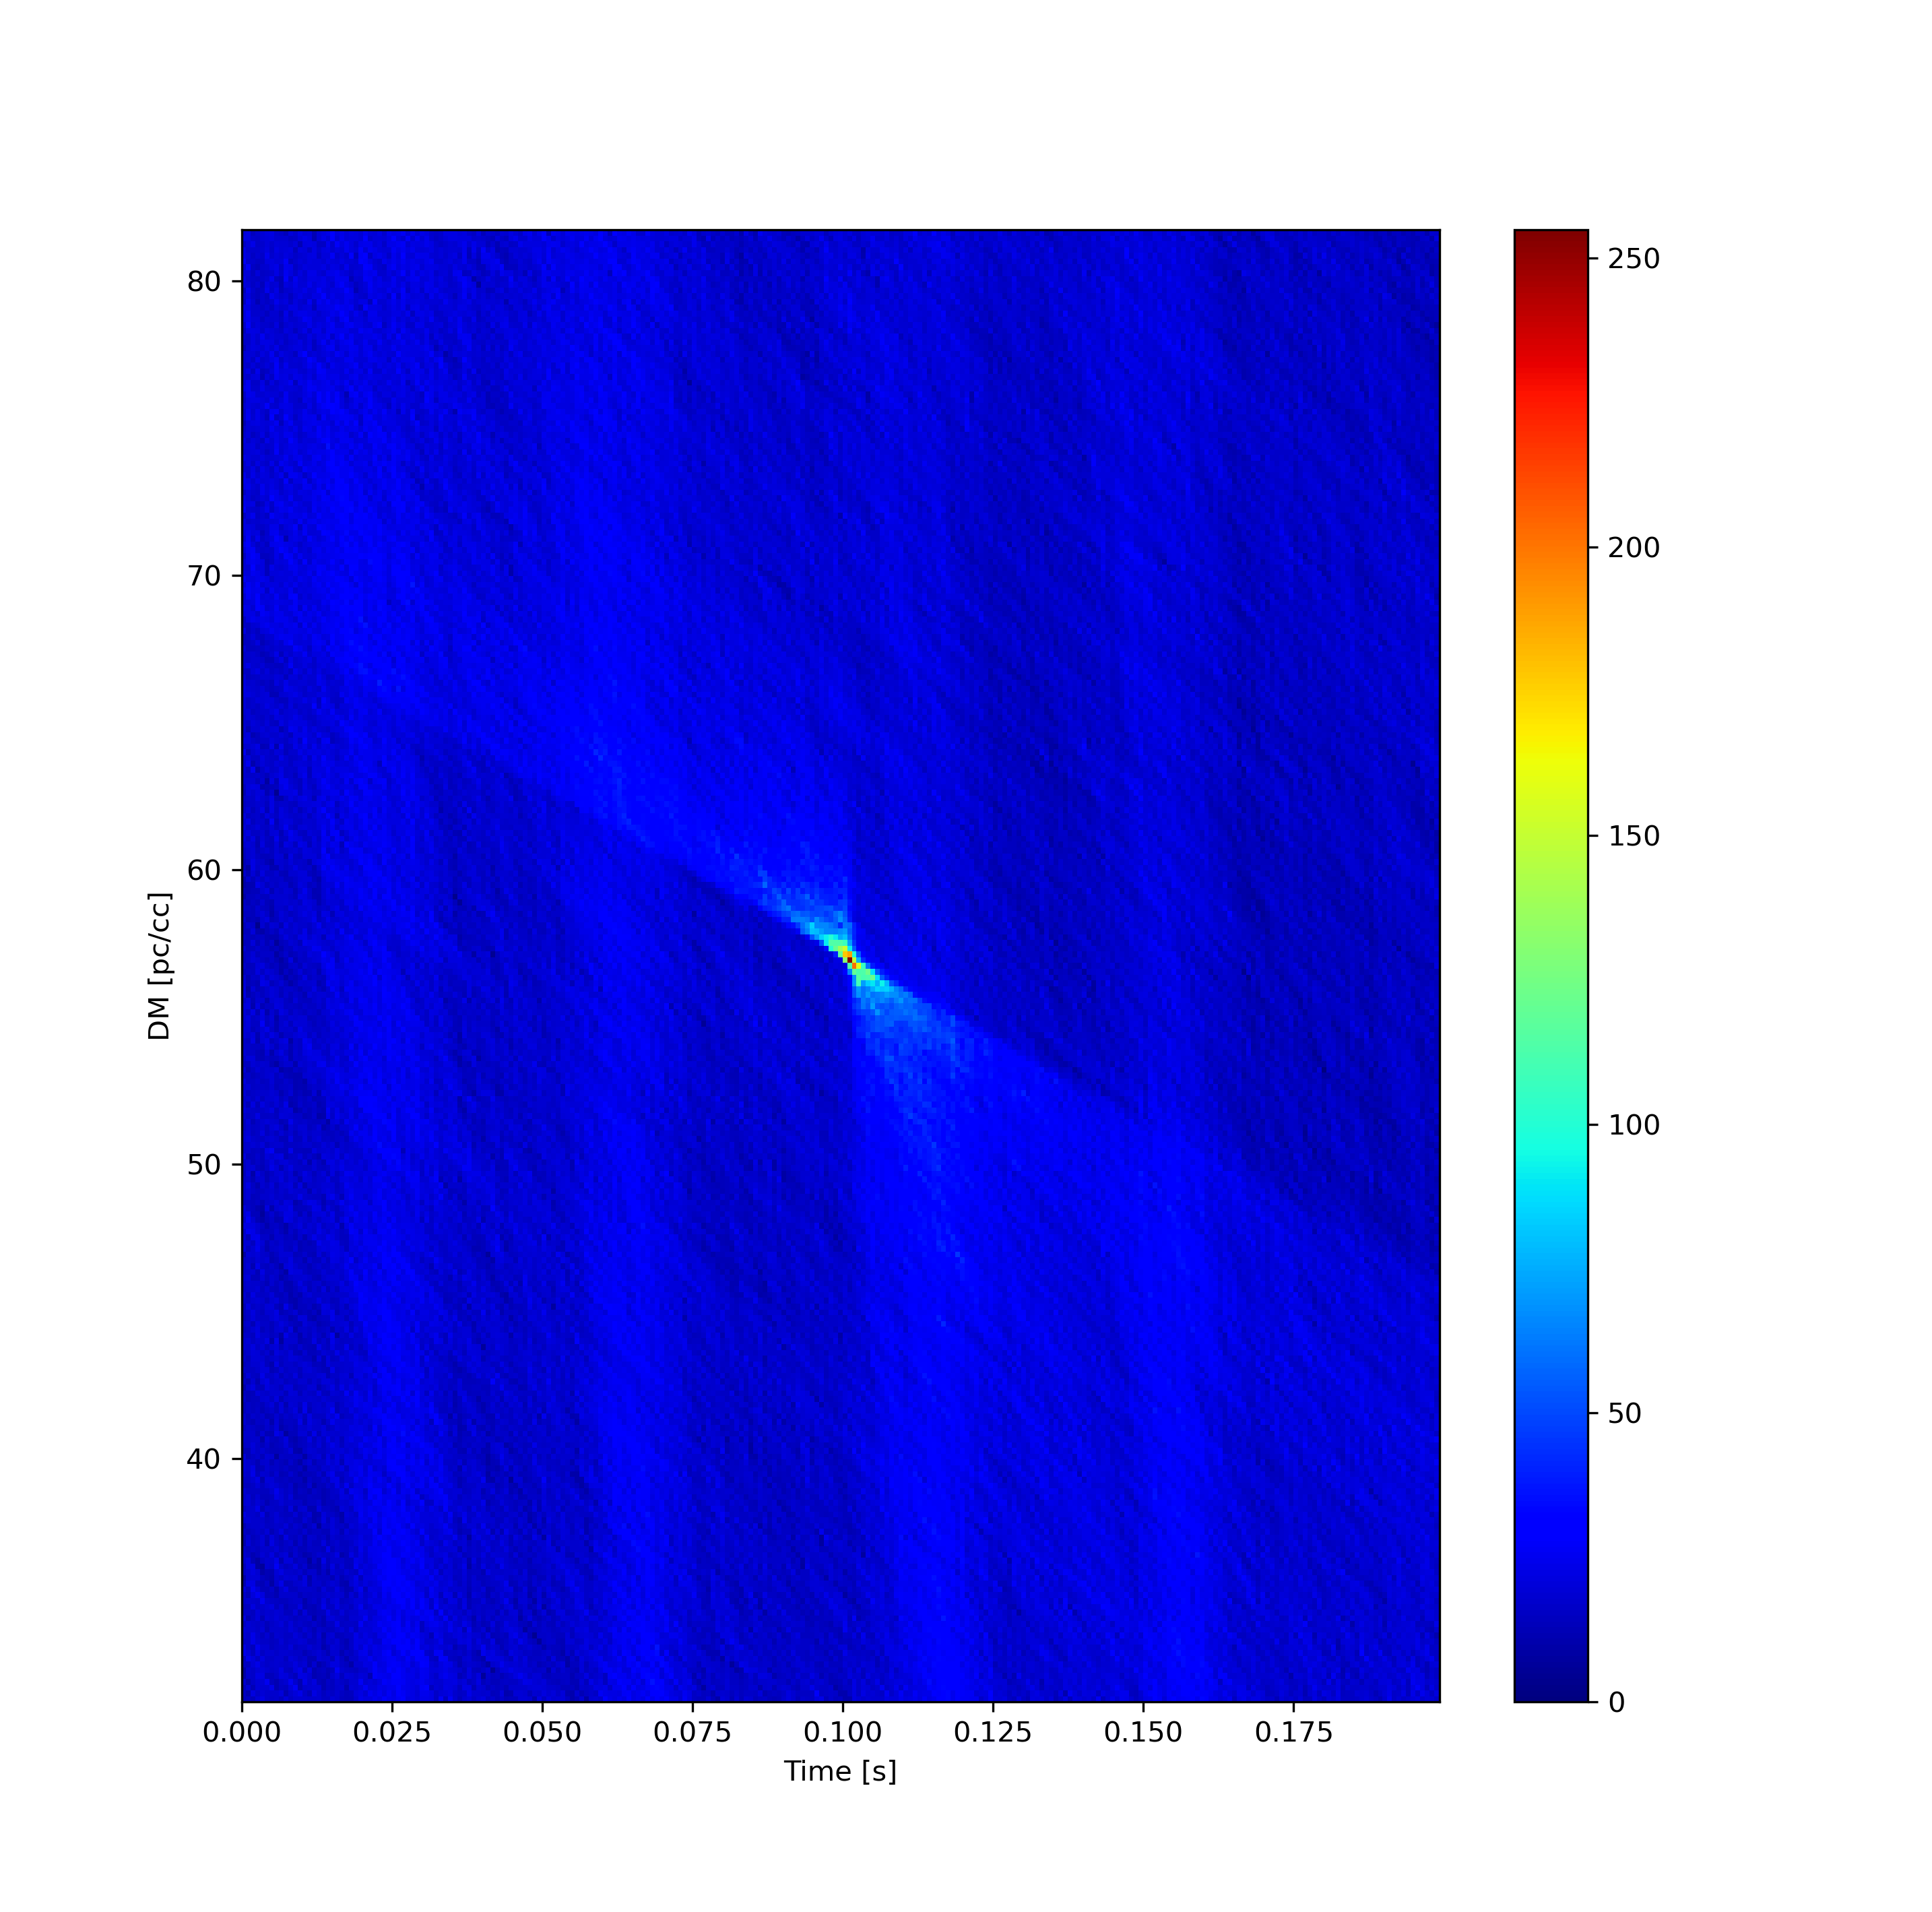
\includegraphics[width=0.8\textwidth, keepaspectratio]{btplane.png}
	\caption{Bowtie plane. \sn as a function of \dm and time. 
	It is called a bowtie plane since a true dispersed signal produces a bowtie.
	This is a trigger from Crab pulsar with \sn$=84.28$ and \dm$=56.75$pc/cc.
	The data is digitized to \texttt{uint8} hence takes integer values in $[0,256)$.
}
\end{figure}

\begin{figure}
	\label{fig:dd}
	\centering
	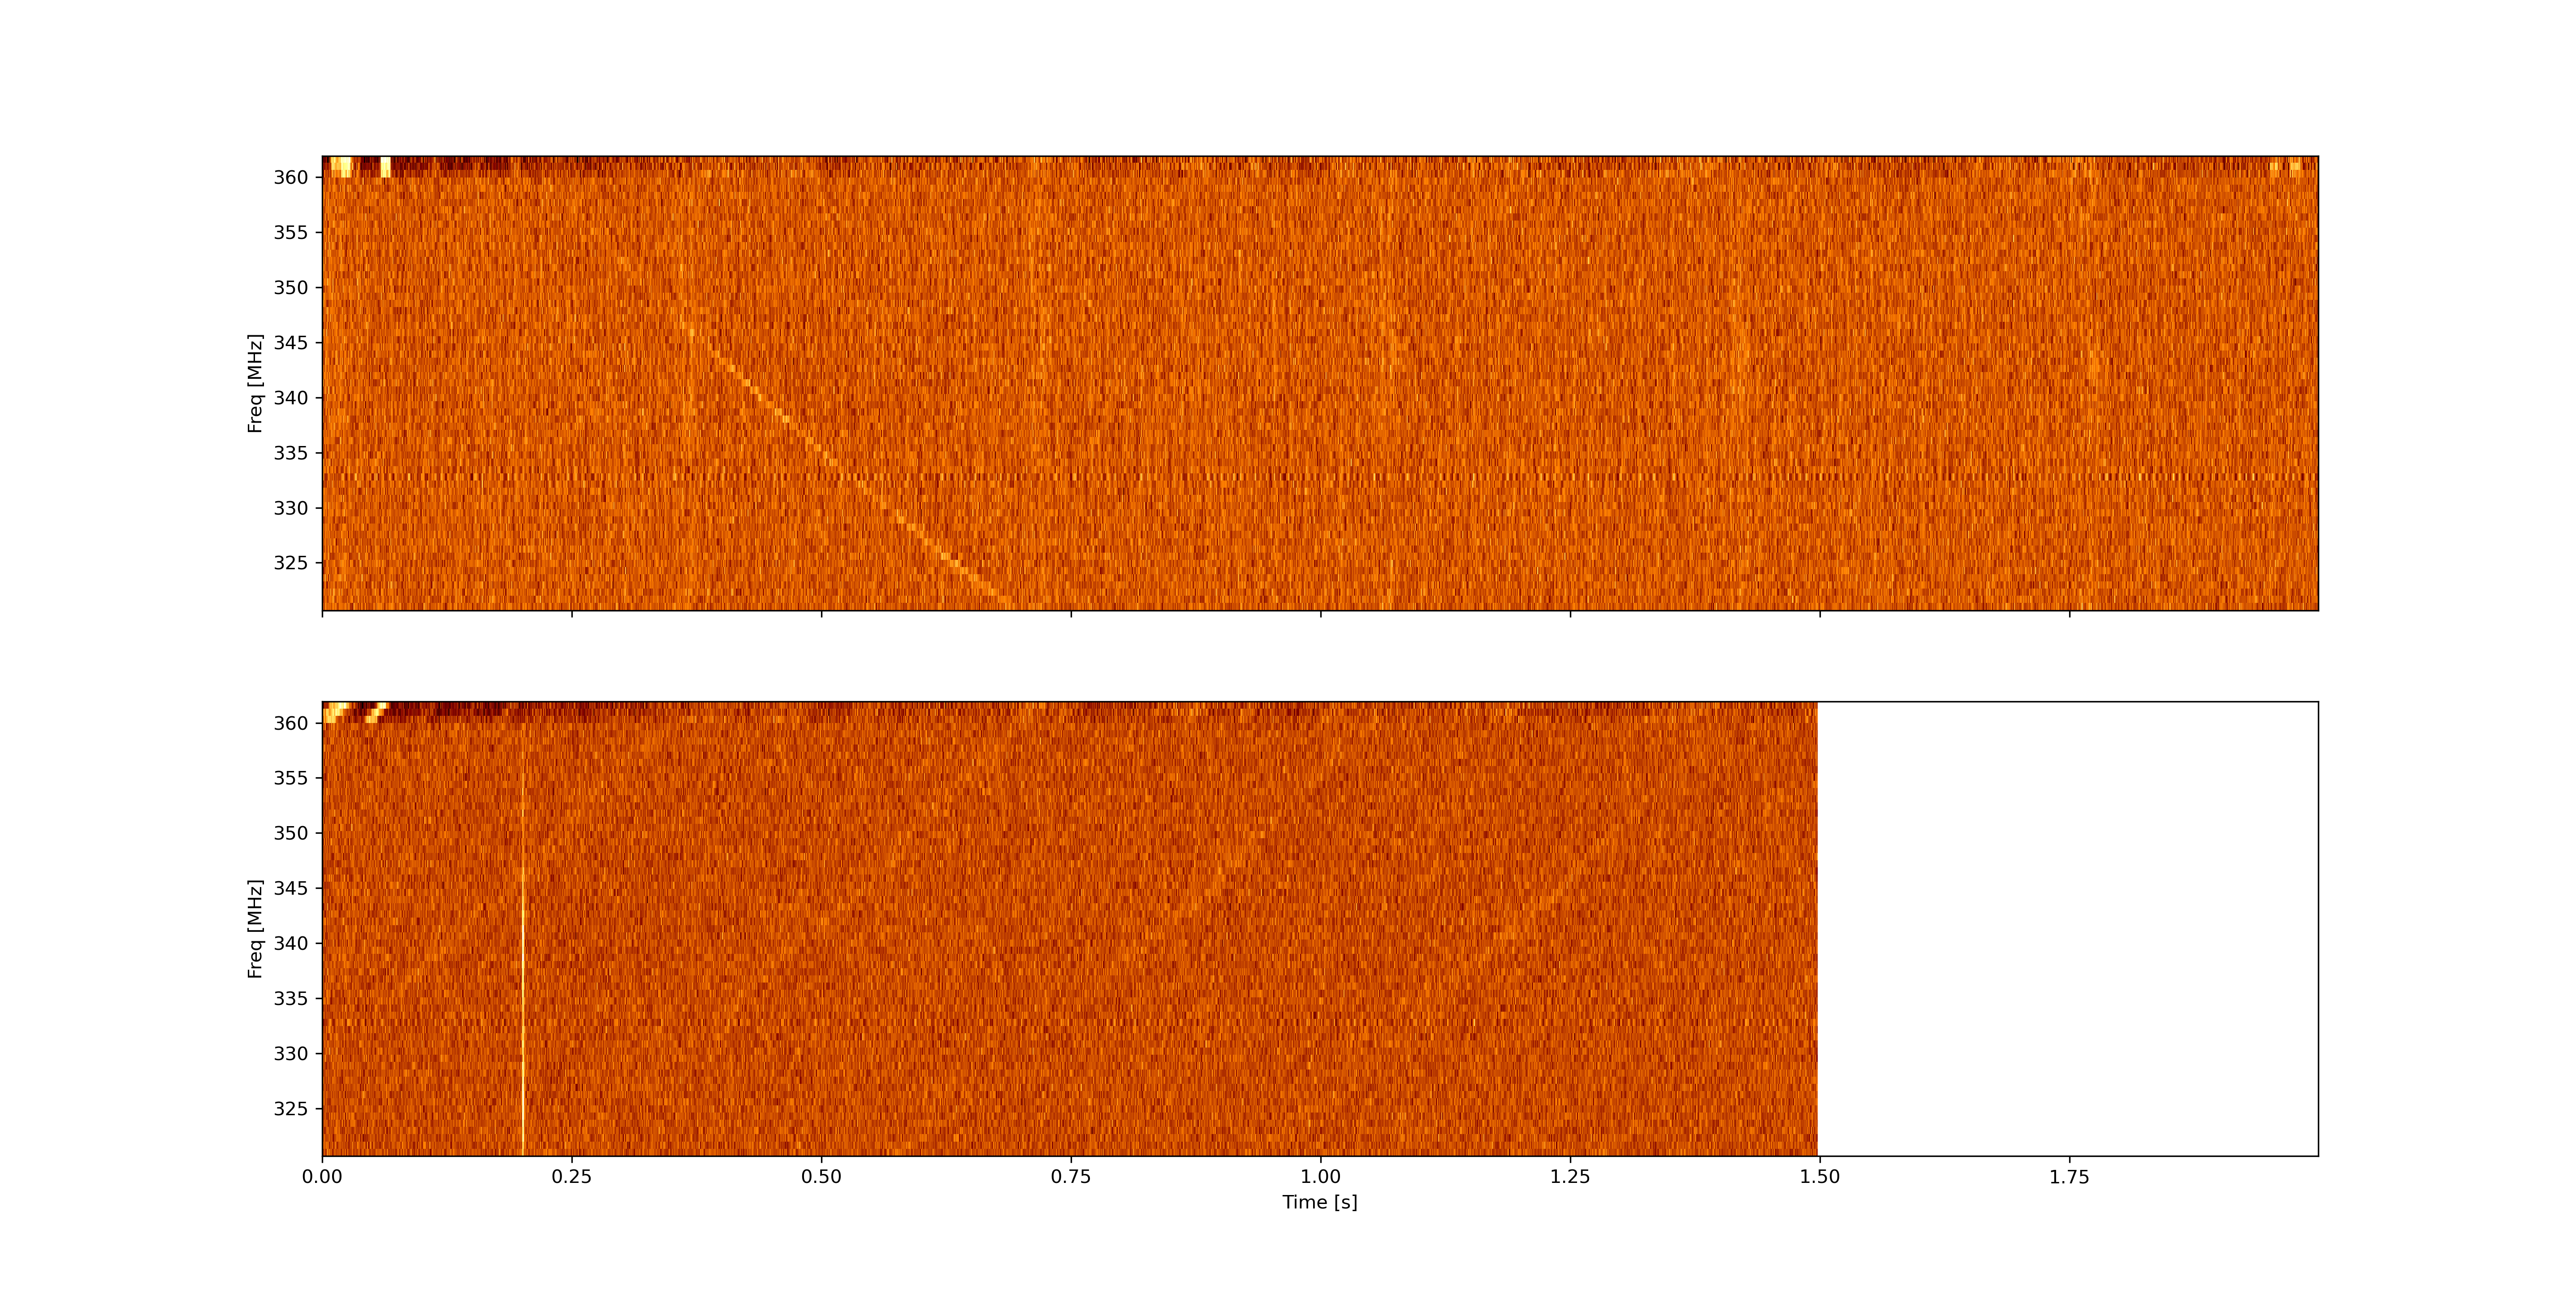
\includegraphics[width=0.8\textwidth, keepaspectratio]{ddidd.png}
	\caption{Top:Dispersed filterbank. Bottom:De-dispersed filterbank.
		Data is from a Crab pulsar trigger with \sn$=8.5$ and \dm$=56.75$pc/cc.
	}
\end{figure}

\subsection {Meta response}
\par For every voltage trigger issued, a variety of meta data has to be packaged to do any kind of analysis with the voltage data. 
This job is performed by Meta response. Meta data involves the following:
\begin{enumerate}
\item Antenna mappings
\item Antenna delays
\item Antenna positions
\item Trigger parameters
\end{enumerate}

\par This job is done by a Python server running on the login node. 
This server listens to the mcast group to which voltage triggers are issued.
For a voltage trigger, it outputs a \textt{metar} file as described in~\autoref{ssub:metar,tab:metar}.

\section {Data products}
\label{sec:datap}
\par This section defines all the data products of the pipeline. 
\subsection {Candidate file}
\label{ssub:candfile}
\par A candidate file consists of tab-separated values. Every new line has either two fields or nine fields. 
The definition of the file is given in~\autoref{tab:candfile}.
% Please add the following required packages to your document preamble:
% \usepackage{multirow}
\begin{table}[]
	\label{tab:candfile}
	\caption{Description of candidate file.}
	\begin{tabular}{lll}
		\begin{tabular}[c]{@{}l@{}}Type of\\ data\end{tabular} & \begin{tabular}[c]{@{}l@{}}Number of\\ fields\end{tabular} & Data                                                                                                                 \\
		\multirow{2}{*}{Pointing}                              & \multirow{2}{*}{2}                                         & Right Ascension in radians                                                                                           \\
																													 &                                                            & Declination in radians                                                                                               \\
		\multirow{9}{*}{Candidate}                             & \multirow{9}{*}{9}                                         & Signal to Noise ratio of the candidate                                                                               \\
																													 &                                                            & \begin{tabular}[c]{@{}l@{}}Index of the first sample of the signal since\\ the start of the observation\end{tabular} \\
																																																									&                                                            & Time of the first sample of signal                                                                                   \\
																																																									&                                                            & Filterwidth of the signal                                                                                            \\
																																																									&                                                            & Index of the DM trial                                                                                                \\
																																																									&                                                            & DM of the signal                                                                                                     \\
																																																									&                                                            & Number of giants in the group                                                                                        \\
																																																									&                                                            & UTC epoch of the start of the signal                                                                                 \\
																																																									&                                                            & UTC epoch of the end of the signal                                                                                  
										 
 \end{tabular}
\end{table}
\begin{table}
	\label{tab:ubson}
	% Please add the following required packages to your document preamble:
	% \usepackage{multirow}
	\begin{tabular}{llll}
		\hline
		Type                        & Parameter   & Present & Comments                                               \\ \hline
																& S/N         & Both    & Signal to Noise ratio of the trigger                   \\
																& DM          & Both    & Dispersion Measure of the trigger                      \\
																& Width       & Both    & Width of the trigger in seconds                        \\
		\multirow{4}{*}{Time}       & Peak time   & Both    & Peak time of the trigger from the start of the data    \\
																	& Tstart      & Both    & MJD of the start of the data                           \\
																	& Tsamp       & Both    & Sampling time of the data                              \\
																	& Duration    & Both    & Duration of the data                                   \\
		\multirow{3}{*}{Frequency}  & Fch1        & Both    & Frequency of the first channel in MHz                  \\
																	& Foff        & Both    & Frequency width in MHz                                 \\
																	& Nchans      & Both    & Number of channels in the data                         \\
		\multirow{4}{*}{Indices}    & I0          & Both    & UTC epoch of the first sample of the data              \\
																	& I1          & Both    & UTC epoch of the last sample of the data               \\
																	& Epoch       & Both    & UTC epoch of the start of the observation              \\
																	& Nsamps      & Both    & Size of the data                                       \\
		\multirow{6}{*}{Parameters} & Nbits       & Both    & Number of bits per datum                               \\
																	& Antenna     & Both    & Station ID                                             \\
																	& Source name & Both    & Name of the source observing when trigger was recorded \\
																	& RA          & Both    & Right Ascension of the source in radians               \\
																	& Dec         & Both    & Declination of the source in radians                   \\
																	& Group       & Both    & String identifier                                      \\
		DMs                         & DM1         & DBSON   & Start DM in pc/cc in bowtie plane                      \\
																& DMoff       & DBSON   & DM width in bowtie plane                               \\
																& NDM         & DBSON   & Number of DM trials in bowtie plane                    \\
		Data                        & FB          & FBSON   & Raw filterbank                                         \\
																& DD          & DBSON   & De-dispersed filterbank                                \\
																& BT          & DBSON   & Bow-tie plane                                          \\ \hline
	\end{tabular}
\end{table}
\subsection {FilterBank jSON}
\par FilterBank jSON (\fbson) is an Universal Binary JSON~\cite{ubjson} file format containing unprocessed filterbank along with header information. Filterbank data is in time major format with frequency index changing the fastest.
The schema is defined in~\autoref{tab:ubson}. 
\par This data product is no longer in use since the trigger processing is currently done in realtime.
\subsection {De-dispersed filterBank jSON}
\label{ssub:dbson}
\par De-dispersed filterbank jSON (\dbson) is an Universal Binary JSON~\cite{ubjson} containing de-dispersed filterbank and bowtie plane digitized to \uchar.
The schema is defined in~\autoref{tab:ubson}.
\subsection {Trigger plot}
\label{ssub:tp}
\par Trigger plot is a diagnostic plot generated for every trigger. 
It is saved in Portable Networks Graphics (PNG,~\cite{png}) format and rendered used PGPLOT~\cite{pgplot} library.

\par A trigger plot consists of bow-tie plane, de-dispersed filterbank, frequency averaged time profile, and \dm profile. 
In addition to them, a trigger plot also shows \sn, width, pointing information, and time information.
A typical trigger plot for a known pulsar trigger is given in~\autoref{fig:tp}.

\begin{figure}
	\label{fig:tp}
	\caption{A trigger plot generated on a trigger realtime. This trigger is from a pulsar.}
\end{figure}

\subsection {META Voltages}
\label{ssub:metar}
\par Meta (\meta) is an Universal Binary JSON~\cite{ubjson} containing meta information required for any voltage analysis.
% Please add the following required packages to your document preamble:
% \usepackage{multirow}
\begin{table}[]
	\label{tab:metar}
	\caption{Schema for Meta dumped for every voltage trigger.}
	\begin{tabular}{lll} \toprule
		Type                     & Parameter      & Comments                                                                                                               \\ \midrule
		\multirow{5}{*}{Header}  & S/N            & Signal to Noise ratio of the trigger                                                                                   \\
														 & DM             & Dispersion Measure in pc/cc of the trigger                                                                             \\
														 & Width          & Width of the trigger in seconds                                                                                        \\
														 & T0             & UTC epoch of the start of the signal                                                                                   \\
														 & T1             & UTC epoch of the end of the signal                                                                                     \\
		\multirow{8}{*}{Delays}  & VLITE\_ANT\_ID & VLITE Antenna ID                                                                                                       \\
														 & VLA Antenna    & VLA Antenna                                                                                                            \\
														 & DIFX\_HOST     & Compute node connected to the antenna                                                                                  \\
														 & DIFX\_IFACE    & Network interface on the compute node                                                                                  \\
														 & CLK\_OFFSET    & Clock offset in nanoseconds                                                                                            \\
														 & PAD            & Antenna string identifier                                                                                              \\
														 & LO\_FIBER      & RF-over-Fiber delay in nanoseconds                                                                                     \\
														 & ENABLE         & If antenna is added to the array                                                                                       \\
		\multirow{7}{*}{Antprop} & CONFIG         & Array configuration identifier                                                                                         \\
														 & DATASETID      & Dataset identifier                                                                                                     \\
														 & CREATION       & Epoch of creation                                                                                                      \\
														 & EOPSET         & \begin{tabular}[c]{@{}l@{}}Earth Orientation Parameter set.\\ TAI\_UTC, UT1\_UTC and \\ pole information.\end{tabular} \\
																																																				& dots           & For each EOPDAY                                                                                                        \\
																																																				& ANTS           & \begin{tabular}[c]{@{}l@{}}Antenna information.\\ WIDAR\_ID, PAD, X, Y, Z, OFFSET\end{tabular}                         \\
																																																																													& dots           & For each antenna                                                                                                      
																																																																								\bottomrule
	\end{tabular}
\end{table}
